\chapter{The TULIPAN Steganogrpahy Algorithm}
\begin{flushright}
\epsfig{file=Images/TulipanLogo.eps,height=3cm}\end{flushright}

\section{Introduction}

In this project we are trying to use a new method for applying ``adaptive stetganography'' without bearing its side effects like 
being ``weakly dependant on the key''. Using TULIPAN, the sender can hide information in an arbitrary JPEG image using ``adaptive steganography'' with no need to send extra information to the recipient about the special manner of distributing secret bits.

In practice, a steganographic scheme is considered secure   fno existing attack can be modified to build a detector that would be
able to distinguish between cover and stego images with a success better than random guessing.

In other adaptive schemes, the adaptively selected components are normally noisy areas or segments with a complex texture. But if the information about the selection is "public" or only “weakly dependent on a key”, the attacker can apply the same rule and start building an attack. So, the adaptive selection does not necessarily improve steganographic security!

This problem with adaptive steganography could be solved if the selection rule is available only to the sender as side information but in principle unavailable to the recipient (and thus any attacker). For example raw, uncompressed image can be used by sender to embed data in JPEG compressed form of it. This idea is generalizied and applied in ``{\it Perturbed Quantization (PQ)}''.

The selection rule is derived from a coding theory problem of transmiting data through a channel which contains a memory with (a large number of) defective cells. To understand better, the idea of selection rule in PQ can be similar to writing on a partly wet paper such that we can write only on the dry parts.  While being sent, the wet part dries out on the way and so nobody (neither the recipient nor the attacker) can distinguish between original wet and dry patterns. 

The benefit of the defective memory code (the wet paper code) is that not only does it give the sender control over the embedding modifications but also enables the sender to communicate to the recipient on average the same number of bits as if the recipient knew the set of dry pixels.

\section{Perturbed Quantization}

Take a raw image $X$ (grayscale as an example). During  JPEG compression for the first time, performing the Discrete Cosine Transform (DCT), a quantization table is used to divide the DCT coefficients by quantization steps; then according to JPEG standards the compression rounds them to integers, finally being encoded to a JPEG file $G$. Assuming $d_i$ and $D_i$ as the DCT coefficients before and after rounding, respectively, we define ``{\it changeable coefficients}'' (dry coefficients) as those coefficients $d_i$ whose fractional part is in a narrow interval around 0.5. That is $d_i - \lfloor d_i \rfloor \in [0.5 - \epsilon, 0.5 + \epsilon ]$.

During compression, we will round changeable coefficients $d_j$ up or down at our will and thus encode up to k bits (k= total number of $d_j$s, 'changeable coefficients') obtaining a compressed and embedded image $G$.

However, we cannot simply code the message bits as LSBs (Least Significant Bit) of the rounded DCT coefficients $D_j$ because the recipient would not know which coefficients carry message bits. We will show later how the sender can communicate on average k bits to the recipient, who has no information about the set of changeable coefficients.

This method, called Perturbed Quantization (PQ), is a method in which during compression we slightly perturb the quantizer (the process of rounding to integers) for a certain subset of changeable coefficients in order to embed message bits.

Here some reasons are given which certify the formidablity of distinguishing “incorrectly” quantized values $D_i$ by an attacker trying to find statistical evidence for it:

\begin{enumerate}
\item The sender is using side information that is practically removed during quantization and is unavailable to the attacker. It is in general impossible for the attacker to reverse JPEG compression and obtain the uncompressed image.
\item Additional selection rule(s) can be established by the sender to decrease the probability of introducing detectable artifacts more and improve the security. For example, to avoid changing coefficients in the areas of the cover image with the attacker's higher prediction probability.
\item The rounding process $d_j \rightarrow D_j$ (quantizing of changable coefficients) has a large stochastic component as a result of the image noise influence on the rounding of changeable coefficients. The authors of~\cite{PQ04} are currently working on a better justification of this heuristic statement in a more exact manner using image models.

\end{enumerate}

\subsection{Information-reducing processes}
Using the idea mentioned above, the sender can slightly modify the numerical values (such as pixel/coefficient/color/index values depending on the format of image $X$) when he is downgrading the digital image (such as using lossy compression, downsizing, quantization, format conversion, recompression, etc.) as he will have access to the values before quantization/rounding is done. So he can repeat the modification whenever he performs any kind of information-reducing process which includes applying quantizers.
 
There are 3 famous examples of image downgrading operations $F$ that could be used for steganography based on PQ: Resizing, Decreasing the color depth by $d$ bits, and JPEG compression. Here, in TULIPAN we only take the advantage of JPEG compression:

{\bf JPEG compression:} For grayscale images, the transformation $T$ maps a square $m_1\times m_2$ matrix of integers $x_{ij}$, into a $m_1\times m_2$ matrix of real numbers $u_{ij}$ in a block-by-block manner. In each $8\times 8$ pixel block $B^x$, the corresponding block $B^u$ in $u_{ij}$ is $DCT(B^x)./q$, where DCT is the 2D DCT transform, q is the quantization matrix, and the operation “./” is an element-wise division. Then the quantizer $Q$ is applied to vector $u$ by coordinates $Q(u_i) = round(u_i)$.

\subsection{Memory with defective cells}
\label{ChapAlgSecPertSubMem}

During this stage, the sender, following some Selection Rule (SR), identifies the set of indices $C \subseteq \{1, ... , n\}$ of coefficeints (or, in general, cover object elements) whose values $u_j, j\in C$, may be perturbed during quantization. As already mentioned above, the sender can, for example, select $u_i$ whose values are close to the middle of the quantization intervals of $Q$:
\begin{eqnarray*}
C = \{i | i \in \{1,..., n\}, u_i \in [L + 0.5 - \epsilon, L + 0.5 + \epsilon] \textrm{ for some integer} L\}. 
\end{eqnarray*}

The tolerance $\epsilon$, should be a small number for example $0.1$. According the selection rule, sender can just modify $u_i$s whose indices are members of $C$ to embed the message inside the image. Now for embedding the message, sender should use the LSB bits of coefficient of $Y = F(X)$ processed image, however they can use the $k$ changeable coefficient but cannot change the $n - k$ wet coefficients. As the recipient does not have any information about the set $C$, this problem is similar to writing in memory with $k$ nondefective and $n - k$ defective cells. As it will be discussed the sender can store on average $k$ bits of the message in such memory.

In our steganogrphic situation, however, the number of defictive cells is so large as in a typical JPEG image, $n \sim 10^6$ and $k \sim 10^4$. The wet paper code is designed to handle such complexity.

\section{Wet Paper Code}
\subsection{Encoder and Decoder}

In the wet paper encoder, generalizing the selection channel idea 
mentioned before, one message bit is embedded as the LSB of a group 
of elements. Assuming q changeable elements in the group, we can 
attempt to embed $q$ message bits by forming $q$ linearly independent linear
combinations of element LSBs instead of just one sum modulo 2 of the 
individual element LSBs to calculate group LSB. Following this, the 
sender and recipient agree on a secret stego key that is used to generate 
a pseudo-random binary matrix $D$ of dimension $q\times n$. Rounding $u_j, 
j\in C$, the sender obtains the column vector $y'$, so that 
the modified binary column vector $b', b'_i = LSB(y_i'), i=1, \dots , n$, 
satisfies
\begin{eqnarray}
 Db' = m
\label{em}
\end{eqnarray} 
at cost of solving a system of linear equations in
GF(2) which is the biggest computational load on the sender.

Using the variable $v=b' - b$ we can rewrite (\ref{em}) to
\begin{eqnarray}
Dv=m-Db
\label{pizza}
\end{eqnarray}
in which there are $k$ unknowns $v_j, j\in C$, while the remaining $n - k$ 
values $v_i, i \notin C$, are zeros. Thus, on the left hand side, we can 
remove from $D$ all $n - k$ columns $i : i\notin C$, and also remove from $v$ 
all $n - k$ elements $v_i$ with $i \notin C$.The system (\ref{pizza}) now 
becomes 
\begin{eqnarray}
Hv = m - Db
\label{salad}
\end{eqnarray}
where $H$ is a binary $q \times k$ submatrix of $D$ and $v$ is an unknown $k\times 1$ 
binary vector. The solvablity of this system of linear equations will be discussed later. 

To decode, having received the modified stego object $Y'=\{y_i'\}$, the 
recipient should only form $b'_i=LSB(y'_i)$ and using shared matrix $D$, 
gets $Db'$ which is the extracted message $m=Db'$.

\subsection{Practical encoder/decoder implementation}
\label{ChapAlgSecWetSubPrac}
The main complexity of this communication setup is on the side of
the sender to solve $q$ linear equations for $k$ unknowns in GF(2). 
Assuming that the maximal length message is sent, the complexity 
of Gaussian elimination for (\ref{salad}) is $O(k^3)$. 
For a medium size image with $n=10^6$ pixels and with $\epsilon=0.1$, 
we have $k \sim 10^4$ for a typical 80\% quality JPEG image. 
While solving a linear system with $10^4$ unknowns using Gaussian 
elimination is doable on a PC, it may require several minutes of 
calculations, which is impractical for the user.

By far the best performance and most flexible method was obtained
using structured Gaussian elimination by dividing the image into $\beta$
pseudo-random disjoint subsets $B_i$ and using the Gaussian elimination on each subset separately. This can bring down the
computational requirements substantially because the complexity of 
Gaussian elimination will decrease by the factor of $\beta^3$ while the 
number of solving increases $\beta$-times.

Keeping the above result in mind, we'll describe the encoder and decoder 
algorithms. $r_2$ is the estimated range of the ratio of the dry to all coefficient
and $h$ is the header size of each matrix. $k_i$ is the number of dry coefficients which are consumed by the $i$-th matrix:

\begin{itemize}
\item {\bf E0.} Using a PRNG, generate a random binary matrix $D$ with $n / \beta$
columns and sufficiently many rows.

\item {\bf E1.} Determine the header size $h=log_2(r_2 n /\beta)+1, q=|m|+ \beta h$

\item {\bf E2.} $b'\leftarrow b,i\leftarrow 1$.

\item {\bf E3.} $q_i=(k_i (q + 10)/k), q_i=min\{q_i,2^h-1,|m|\}, m^{(i)}\leftarrow \textrm{the next } q_i \textrm{ bits in } m$

\item {\bf E4.} Select the first $n_i$ columns and $q_i$ rows from $D$ and denote this submatrix $D^{(i)}$. Solve $q_i$ equations $H^{(i)}v=m(i) - D^{(i)}b^{(i)}$ for $k_i$ unknowns $v$, where $H(i)$ is a $q_i\times k_i$ submatrix of $D^{(i)}$ consisting of those columns of $D^{(i)}$ that correspond to changeable bits in $B_i$. If this system does not have a solution, the encoder decreases $q_i$ till a solution is found.

\item {\bf E5.} According to the solution vector $v$, obtain the $i$-th segment $b'^{(i)}$ of the vector $b'$ by modifying or leaving $b^{(i)}$ unchanged.

\item {\bf E6.} Binary encode $q_i$ using $h$ bits and append them to $m$.

\item {\bf E7.} Remove the first $q_i$ bits from $m$.

\item {\bf E8.} $q \leftarrow q - q_i, k \leftarrow k - k_i, i\leftarrow i+1$.

\item {\bf E9.} If $i < \beta$ GOTO E3.

\item {\bf E10.} If $i=\beta , q_\beta \leftarrow q$.

\item {\bf E11.} Binary encode $q_\beta$ using $h$ bits and prepend to $m$, $m^{(\beta)}\leftarrow m$.

\item {\bf E12.} Select the first $n_{\beta}$ columns and $q_{\beta}$ rows from $D$ and denote this submatrix $D^{(\beta)}$. Solve $q_{\beta}$ equations $H^{(\beta)}v=m^{(\beta)}-D^{(\beta)}b^{(\beta)}$ for $k_{\beta}$ unknown $v$s. If this system does not have a solution, exit and report failure to embed the message.

\item {\bf E13.} According to the solution $v$, obtain the $\beta$-th segment $b'^{(\beta)}$ of the vector $b'$ by modifying or leaving $b^{(\beta)}$ unchanged.

\end{itemize}

The Decoder Algorithm is as follows:

\begin{itemize}

\item {\bf D0.} Using a PRNG, generate a random binary matrix $D$ with $n/\beta$ columns and sufficiently many rows.

\item {\bf D1.} Determine the header length $h=log_2(r_2n/\beta)+1$.

\item {\bf D2.} $i\leftarrow\beta$.

\item {\bf D3.} Select the first $n_\beta$ columns and $h$ rows from $D$ and denote this submatrix $D_h$. Obtain $h$ bits as $D_hb'^{(\beta)}$ and decode as $q_\beta$

\item {\bf D4.} Select the first $n_\beta$ columns and next $q_\beta - h$ rows from $D$ and denote this submatrix $D^{(\beta)}$. Obtain message bits $m=D^{(\beta)}b'^{(\beta)}$.

\item {\bf D5.} $i\leftarrow i - 1$

\item {\bf D6.} Decode $q_i$ from the last $h$ bits of $m$ and remove the last $h$ bits from $m$.

\item {\bf D7.} Select the first $n_i$ columns and $q_i$ rows from $D$ and denote this submatrix $D^{(i)}$. Prepend $D^{(i)}b'^{(i)}$ to $m$, $m \leftarrow D^{(i)}b'^{(i)}\& m$.

\item {\bf D8.} If $i > 1$ GOTO 5
\item {\bf D9.} ELSE $m$ is the extracted message.

\end{itemize}

\section{Average Capacity}

As it was discussed in previous section, the ability of the sender to encode a $q$ bit message, depends on solvablity of $q\times k$ matrix H. That system has a solution for an arbitrary message $m$ as long as $rank(H) \geq q$. The elegant result on which wet paper code is based, is that for large $k$ the probability that the rank of a random $q \times k$ binary matrix becomes maximum (equal to k), quickly approaches $1$ as $q$ increases slightly more than $k$. This result is shown in Figure~\ref{ChapAlgSecCapFigProb}.

\begin{figure}
\begin{center}
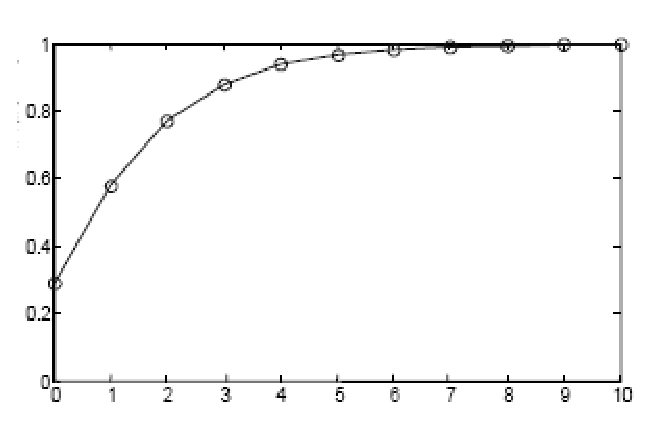
\epsfig{file=Images/FullRankProbability.eps}
\caption{Probability that a random $q \times k$ binary matrix has
  rank $k$ (for large $k$). The x axis indicates $q - k$.}
\label{ChapAlgSecCapFigProb}
\end{center}
\end{figure}

This means that on average, the sender will be able to communicate k bits to the recipient using the wet paper code.

\section{Double Compression}
In TULIPAN we use the PQ embedding method based on double compression. The method takes a (single compressed) JPEG file as the cover image and produces a double compressed JPEG file as the stego image. The sender and recipient can use the LSB of DCT to embed the message. The sender chooses the second quality factor $Q2 < Q1$ (to make the recompression information-reducing) to derive some dry coefficients in the downgraded image. During the quantization process of the lower quality image, the sender enforces that the quantized value ($D_{j}$) of the $d_{j}$ changeable DCT coefficient in the stego file to be either $l$ or $l+1$ according to the encoded message bit and stores it as the value of the quantized $D_{j}$ DCT coefficient in the stego image.

The numerical experiments on downgrading the JPEG images qualities indicates that if the sender sets the second quality according to
\begin{eqnarray}
Q2 = 2(Q1 - 50)
\end{eqnarray}

The number of changeable coefficient increase to about the maximum. This result is depicted in Figure~\ref{ChapAlgSecDoubleFigCap}.

\begin{figure}
\begin{center}
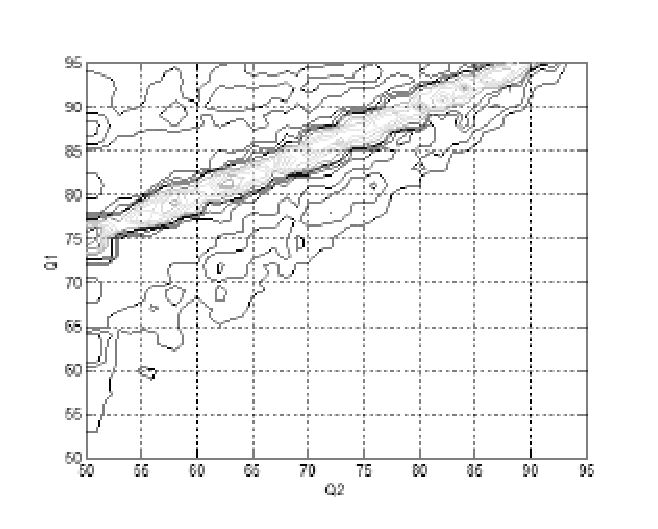
\epsfig{file=Images/DoubleCompressionCapacity.eps}
\caption{Embedding capacity expressed in bits per non-zero DCT coefficient (of the double-compressed image) averaged over 20 test images. Note the prominent ridge for quality factors satisfies $Q2 = 2(Q1 - 50)$.} 
\label{ChapAlgSecDoubleFigCap}
\end{center}
\end{figure}

\section{Steganalysis}
An steganalysis on a bulk of gray scale images has been done using a blind steganlayzer. Random messages of various length (0.4, 0.2, 0.1, and 0.05 bits per non-zero DCT coefficient of the stego image)  were embedded into a subset of these images using 6 modern steganographic schemes, F5, F5 without matrix embedding, OutGuess, Model based Steganography without and with deblocking and PQ. Then the detection reliability factor of the blind steganalyser is calculated for detecting the existence of message inside the image. The detection reliablity factor of ``0'' means complete random detection and the complete defeat of the steganalyzer. On the other hand, the detection reliablity factor of ``1'' means that the steganalyzer can distinguish the stego images from the ordinary images perfectly. The result of this experiment is shown in Table~\ref{ChapAlgSecStegTabComp}.

\begin{table}
\begin{center}
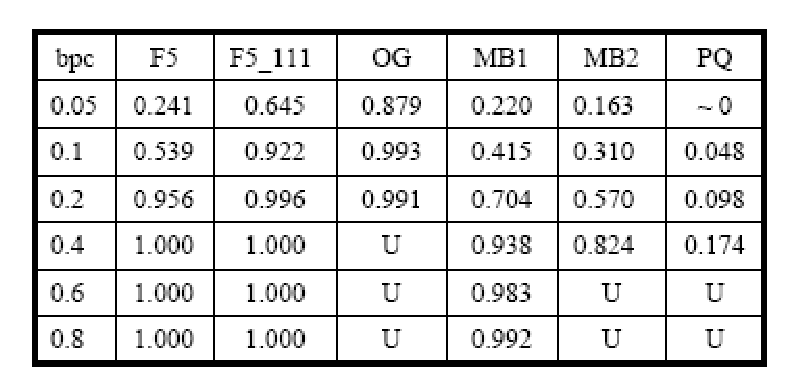
\epsfig{file=Images/SteganalysisComparison.eps}
\caption{Detection reliability  for F5, F5 without matrix embedding (1,1,1), OutGuess 0.2 (OG), Model based Steganography without and with deblocking (MB1 and MB2, respectively), and the proposed Perturbed Quantization during double compression for different embedding rates (U =
unachievable rate). All but the PQ algorithm, were tested with Q = 80. The PQ algorithm was tested with Q1 = 85 and Q2 = 70.} 
\label{ChapAlgSecStegTabComp}
\end{center}
\end{table}

As can be seen from Table~\ref{ChapAlgSecStegTabComp}, the PQ algorithm significantly outperforms existing steganographic algorithms for JPEG images. 

\section{Discussion and Conclusions}

For implementing TULIPAN we used PQ algorithm as it showed the best result from the aspect of security. This result was predictable prior to  implementation due to the brand new idea of adaptive stegonography with side information totally unknown by the recipient and the attacker. 

However, as the idea is new and independent of the idea of other steganographic schemes, The designers of TULIPAN hope that they can employ other steganographic methods combined by PQ to increase its security.